\chapter{Data Validation}

\section{WBPCB}

\textbf{West Bengal Pollution Control Board} (WBPCB) keeps tracks of the pollutant data in some of the cities in the state. This is conducted at various monitoring stations in the state and near the polluting clusters of industries. Specific parameters like Oxides of Sulfur, Oxides of Nitrogen, Respirable Particulate Matter etc. are monitored in the ambient air quality monitoring stations. Data of ambient air quality monitoring stations are presented at the web site of the Board (http://www.wbpcb.gov.in/). \\

WBPCB has their monitoring station in our city of Durgapur too. The station is situated Sidhu Kanhu Indoor Stadium, Recol Park, city Centre, Durgapur, West Bengal 713216.(Coordinates : 23°32'25"N   87°17'29"E)

\vspace{0.1in}

\begin{figure}[!htbp]
	\centering
	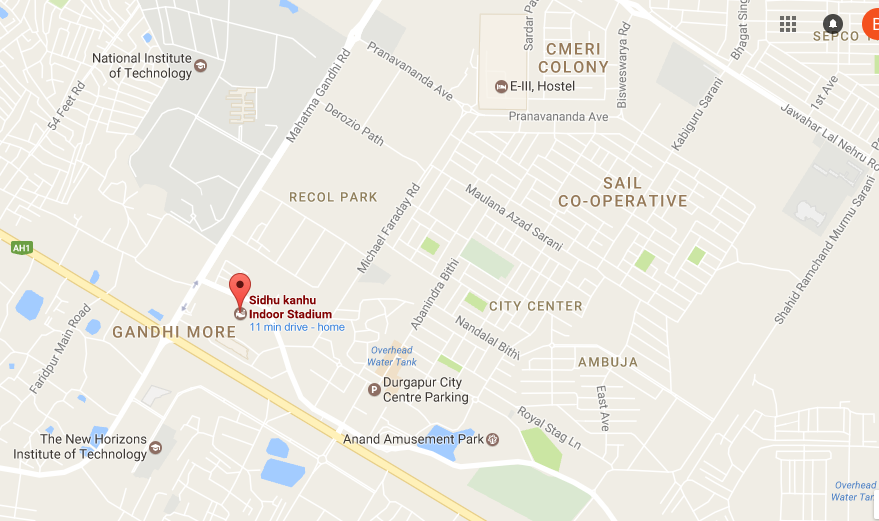
\includegraphics[width=0.7\textwidth]{wbpcb.png}
	\label{fig:Map showing location of WBPCB Stations}
	\caption{Map showing location of WBPCB Stations}
\end{figure}

WBPCB is using sampling based technology to keep track of the pollutants and they upload the hourly data of the area However our Box uses a sensor based technology for the same.\\

\textbf{They are monitoring concentration of pollutants which are Particulate Matter size 10 Micron(PM10), Nitrogen Dioxide (NO2), Sulphur dioxide (SO2), Carbon Monoxide (CO) and Ozone (O3).}.
The pollutants concentration data coming from the Environment Monitoring Box is validated against the WBPCB monitored data to check the efficiency of the data. This process in also called \textbf{Soft Calibration}.

\section{Deployment}

We have deployed our Environment Monitoring Box near to the WBPCB station in Durgapur. The deployment site is 300 m away from the WBPCB station.The box is deployed in the roof top of Pinacle Infotech, Near Junction Mall, City Centre, Durgapur, West Bengal.

\vspace{0.2in}

\begin{figure}[!htbp]
	\centering
	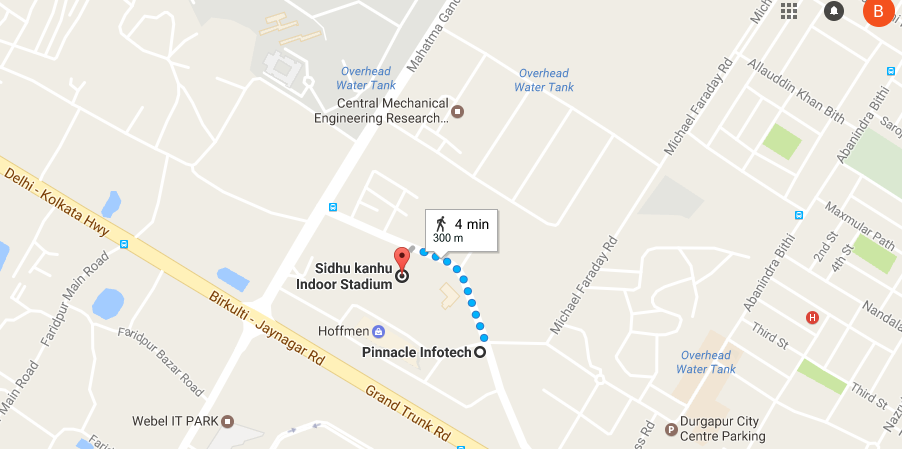
\includegraphics[width=0.9\textwidth]{deployment.png}
	\label{fig:Map showing Our EMB deployment site near to WBPCB station}
	\caption{Map showing Our EMB deployment site near to WBPCB station}
\end{figure}

\vspace{0.1in}
We have taken the reading for 24 hours duration. I.e.17TH May 2017, 12:00 PM to 18TH May 2017, 12:00 PM.

\section{Results and Analysis}
As Mentioned above, the WBPCB station data give the value for (PM10, CO, NO2, SO2), So we have validated the box for (PM10,CO and NO2) only, as we were not having SO2 at the time.
Also The WBPCB station is giving hourly data but our Box is giving data per second so we have calculated mean of the data of the box.
\\
Also we have selected ppm as a unit for measurement of CO and NO2 but WBPCB station gives the data in unit of(mg/m\textasciicircum3) . So we needed to convert.

\subsection{Conversion Formula for ppm(parts per Million) to mg/$m^3$}

mg/$m^3$ = (ppm*molecular weight )/24.45
\\
\\
Here, Molecular weight belongs to individual gases. 

Molecular weight for NO2 is 46.01.

Molecular Weight for CO is 28.01.

\subsection{Plots}
After Collecting the data from WBPCB website for the above said dates and time and from our Box.
The data is labelled as WBPCB for WBPCB station data and BOX for our Box data.

The comparison plots for CO, NO2 and PM10 are:


\begin{figure}[!htbp]
	\centering
	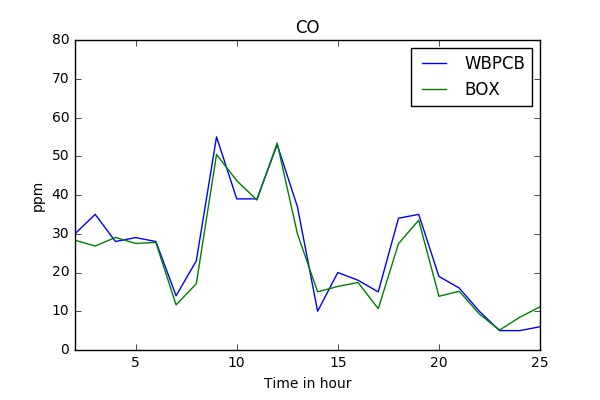
\includegraphics[width=0.9\textwidth]{co.jpg}
	\label{fig:Comparison of CO data}
	\caption{Comparison of CO data}
\end{figure}

\begin{figure}[!htbp]
	\centering
	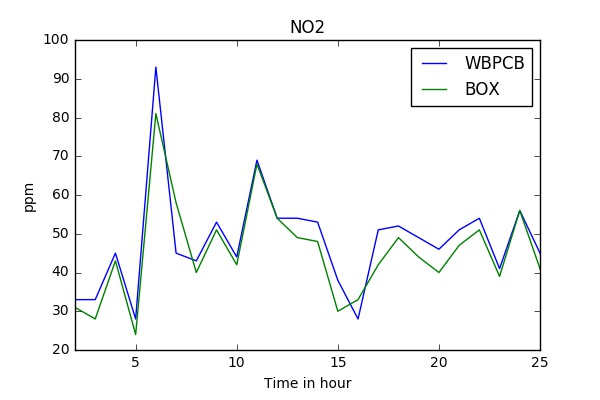
\includegraphics[width=0.9\textwidth]{no2.jpg}
	\label{fig:Comparison of NO2 data}
	\caption{Comparison of NO2 data}
\end{figure}

\begin{figure}[!htbp]
	\centering
	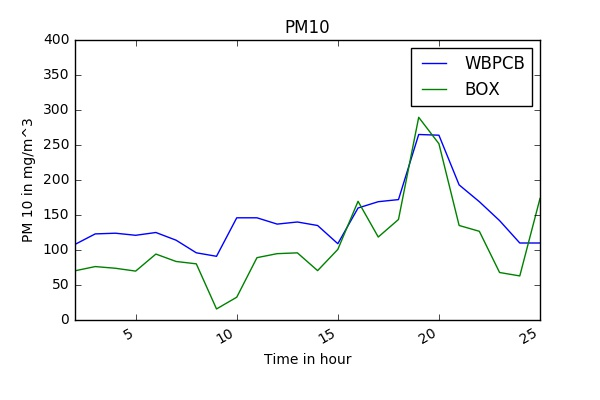
\includegraphics[width=0.9\textwidth]{pm10_compare.jpg}
	\label{fig:Comparison of PM 10 data}
	\caption{Comparison of PM 10 data}
\end{figure}

The Mean difference between the reading of WBPCB station data and our box data is summarized in the following table

\begin{figure}[!htbp]
	\centering
	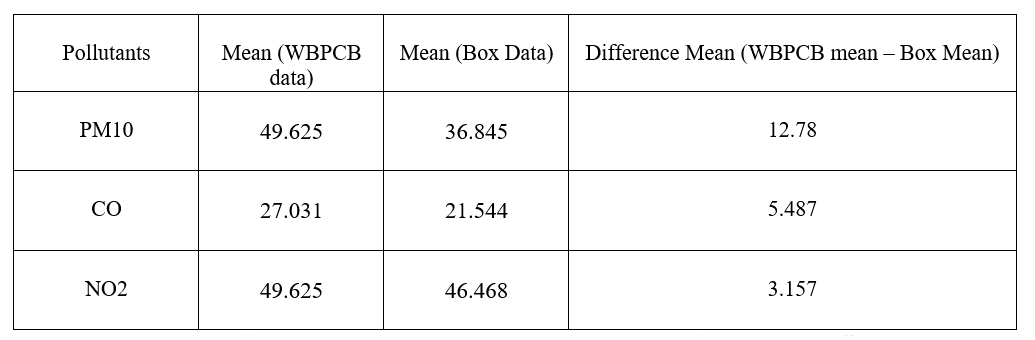
\includegraphics[width=0.9\textwidth]{table.jpg}
	\label{fig:Table showing Mean difference between the Data from WBPCB station and Box data for different pollutants}
	\caption{Table showing Mean difference between the Data from WBPCB station and Box data for different pollutants}
\end{figure}

\newpage
\section{Inferences}

The following conclusion can be drawn from the Plots:

\begin{enumerate}
	\item The Range of our data is same as that of WBPCB for all the three pollutants
	\item Though the value is exactly not same but it is very close to the reading of the WBPCB station (which is high quality sampling based system).
	\item The signature of the curves are same which signifies that our Box is able to catch the variations of data.
\end{enumerate}